\section{Fan Coil Unit (FCU)}
\label{sec:fcu}
%\fbox{LIU: OpenModelica Room and Wall FMUs not available.}

\subsection{Example Description}

This example is inspired by the Heating Ventilation and Air Conditioning (HVAC) industrial case study developed in Task T1.3. The Fan Coil Unit~(FCU) aims to control the  air temperature in a room through the use of several physical components and software controllers. Water is heated or cooled in a \emph{Heat Pump} and flows to the \emph{Coil}. A \emph{Fan} blows air through the \emph{Coil}. The air is heated or cooled depending upon the \emph{Coil} temperature, and flows into the room. A \emph{Controller} is able to alter the fan speed and the rate of the water flow from the \emph{Heat Pump} to the \emph{Coil}.  In addition, the room temperature is affected by the walls and windows, which constitute the environment of the FCU.

The aim of the system is to maintain a set temperature in the single room in which the FCU is located. The system is outlined in Figure~\ref{fig:fcuoverview}.

\begin{figure}[htbp]
\begin{center}
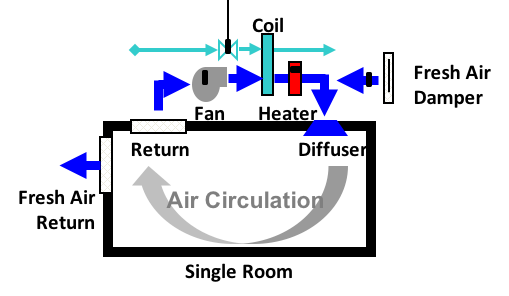
\includegraphics[width=0.6\textwidth]{fcu/fcu_overview}
\caption{Overview of the fan coil unit (FCU) example}
\label{fig:fcuoverview}
\end{center}
\end{figure}

\subsection{Usage}
\label{sec:fcu_usage}

The example is available from the INTO-CPS application menu at \emph{File>Import Example Project} or at \url{https://github.com/INTO-CPS-Association/example-fcu} in the \emph{master} branch. There are several subfolders for the various elements: DSEs - contains various work in progress DSE scripts to alter CT and DE parameters; \texttt{FMU} contains the various FMUs of the study; \texttt{Models} -- contains the constituent models defined using the INTO-CPS simulation technologies; \texttt{Multi-models} -- contains the multi-model definitions and co-simulation configurations; \texttt{SysML} -- contains the SysML model defined for the study; \texttt{resources} -- various images for the purposes of the readme file; and \texttt{userMetricScripts} -- contains files for DSE analysis. 

The \texttt{case-study\_fcu} folder can be opened in the INTO-CPS application to run the various co-simulations as detailed in this document. To run a simulation, expand one of the multi-models and click `Simulate' for an experiment. 

%\subsection{INTO-CPS Technology}
%
%The demonstration on INTO-CPS technologies with the FCU example concentrates on the INTO-CPS SysML profile, shown in Section~\ref{sec:fcu_into_sysml}

\subsection{INTO-CPS SysML Profile}
\label{sec:fcu_into_sysml}

%\subsubsection*{3-model Version}
%Two versions of the FCU model are defined using the INTO-CPS SysML profile. The first corresponds to the architecture used in the baseline OpenModelica and Crescendo models. In this version, t
Three constituent parts are defined -- shown in Figure~\ref{fig:fcu_sysml_asd}:  the \emph{RoomHeating} subsystem, a \emph{Controller} cyber component and the physical \emph{Environment}. The first is a continuous subsystem and comprises the \emph{Room} and \emph{Wall} components.  The figure defines the model platform to be 20-sim, however, this could be OpenModelica too. All of the physical elements of the system are contained in a single CT model. The controller subsystem is a cyber element and modelled in VDM-RT.

\begin{figure}[htb!]
\begin{center}
     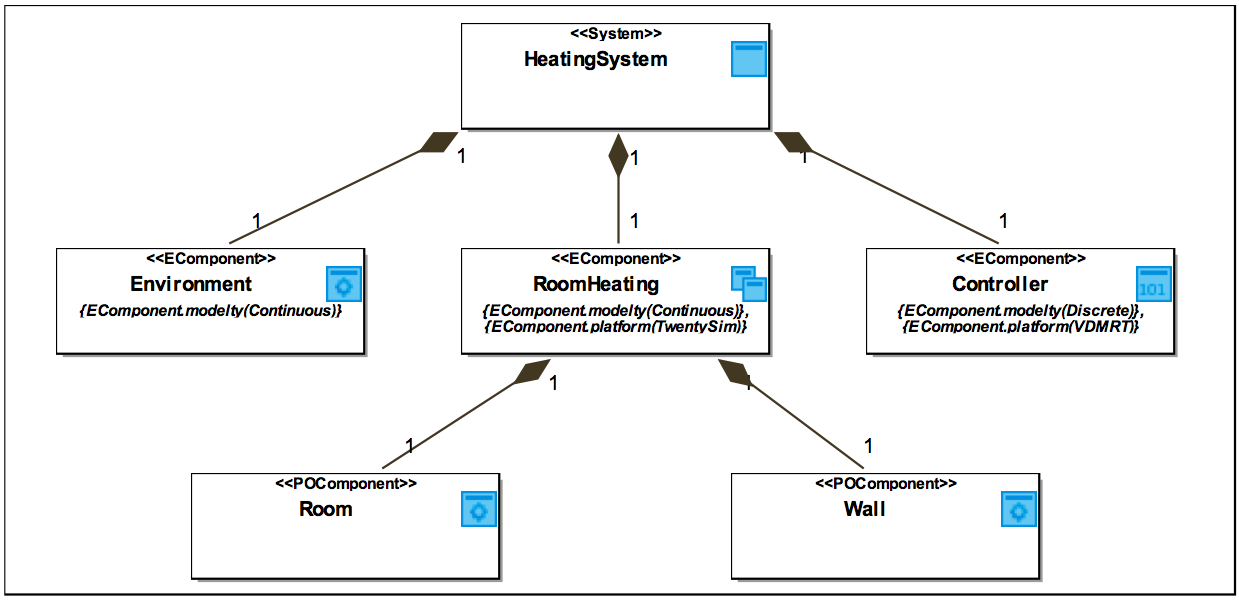
\includegraphics[width=0.75\linewidth]{fcu/fcu_sysml_asd}
\caption{SysML Architecture Structure Diagram using INTO-CPS profile corresponding to baseline models}
\label{fig:fcu_sysml_asd}
\end{center}
\end{figure}

The connections between components, shown in Figure~\ref{fig:fcu_sysml_cd}, are similar to those in the baseline CT models, although it should be noted that the subsystem hierarchy is shown, with the \emph{Room} component supplying and receiving the flows of the \emph{RoomHeating} subsystem.
The connections between CT and DE models show the interface that is managed during the co-simulation. Specifically, the Room Air Temperature (\emph{RAT}) from the CT system is communicated to the controller, which sets the fan speed \emph{fanSpeed} and the valve open state \emph{valveOpen} used by the Room component model \emph{r}, with the aim of achieving the Room Air Temperature Set Point \emph{RATSP} provided by the user in the \emph{Environment}. 

\begin{figure}[htb!]
\begin{center}
     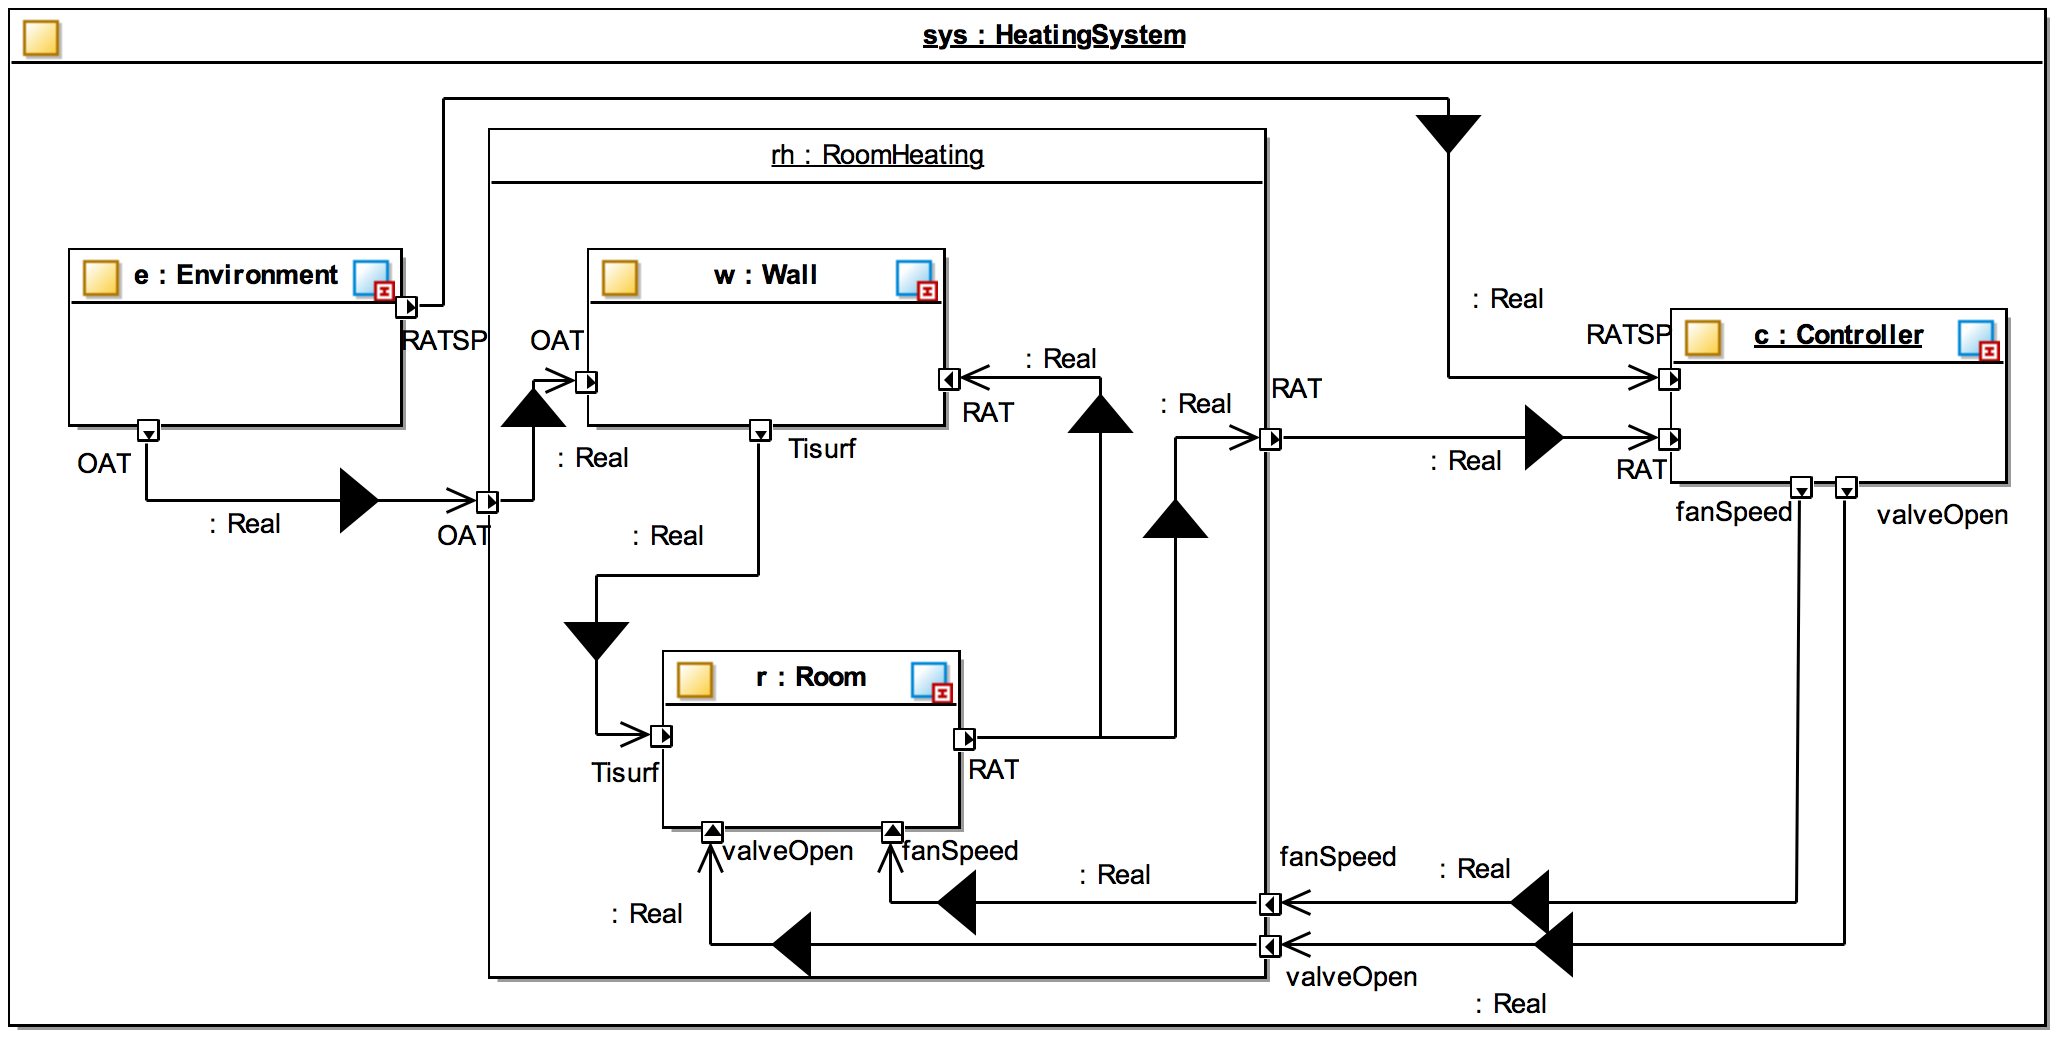
\includegraphics[width=0.7\linewidth]{fcu/fcu_sysml_cd}
\caption{SysML Connection Diagram using INTO-CPS profile corresponding to baseline models}
\label{fig:fcu_sysml_cd}
\end{center}
\end{figure}

%\subsubsection*{4-model Version}
%
%Moving to a more `pure' multi-modelling approach, the next model proposes an alternative subsystem structure. In this model, the ASD in Figure~\ref{fig:fcu_sysml_mm_asd} shows the HeatingSystem comprises four subsystems; the components comprising the \emph{RoomHeating} subsystem in Figure~\ref{fig:fcu_sysml_asd} are lifted to be top-level components in their own right. 
%
%\begin{figure}[htb!]
%\begin{center}
%     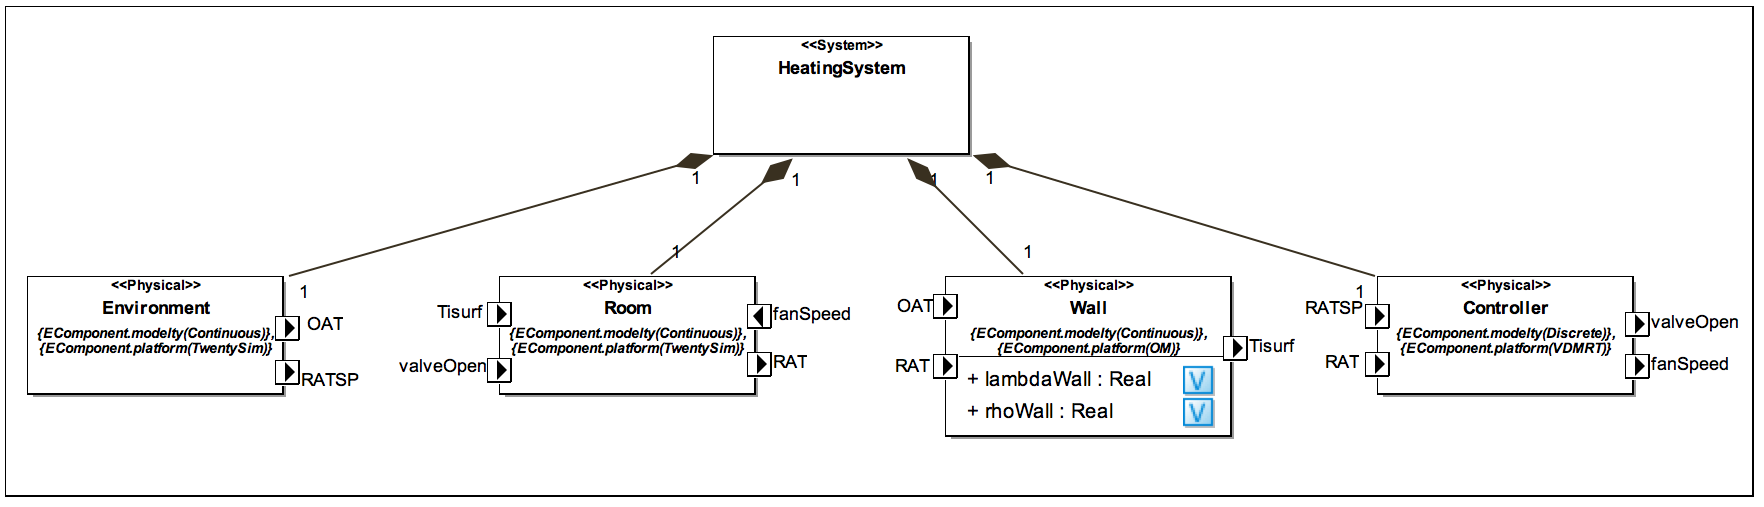
\includegraphics[width=1\linewidth]{fcu/fcu_sysml_asd_mm}
%\caption{SysML Architecture Structure Diagram using INTO-CPS profile corresponding to the `pure' multi-model approach}
%\label{fig:fcu_sysml_mm_asd}
%\end{center}
%\end{figure}
%
%This is reflected in the CD in Figure~\ref{fig:fcu_sysml_mm_cd}, with direct connections between the elements. Each of the CT components (\emph{Room}, \emph{Wall} and \emph{Environment}) may now be modelled in different notations.
%
%\begin{figure}[htb!]
%  \begin{center}
%     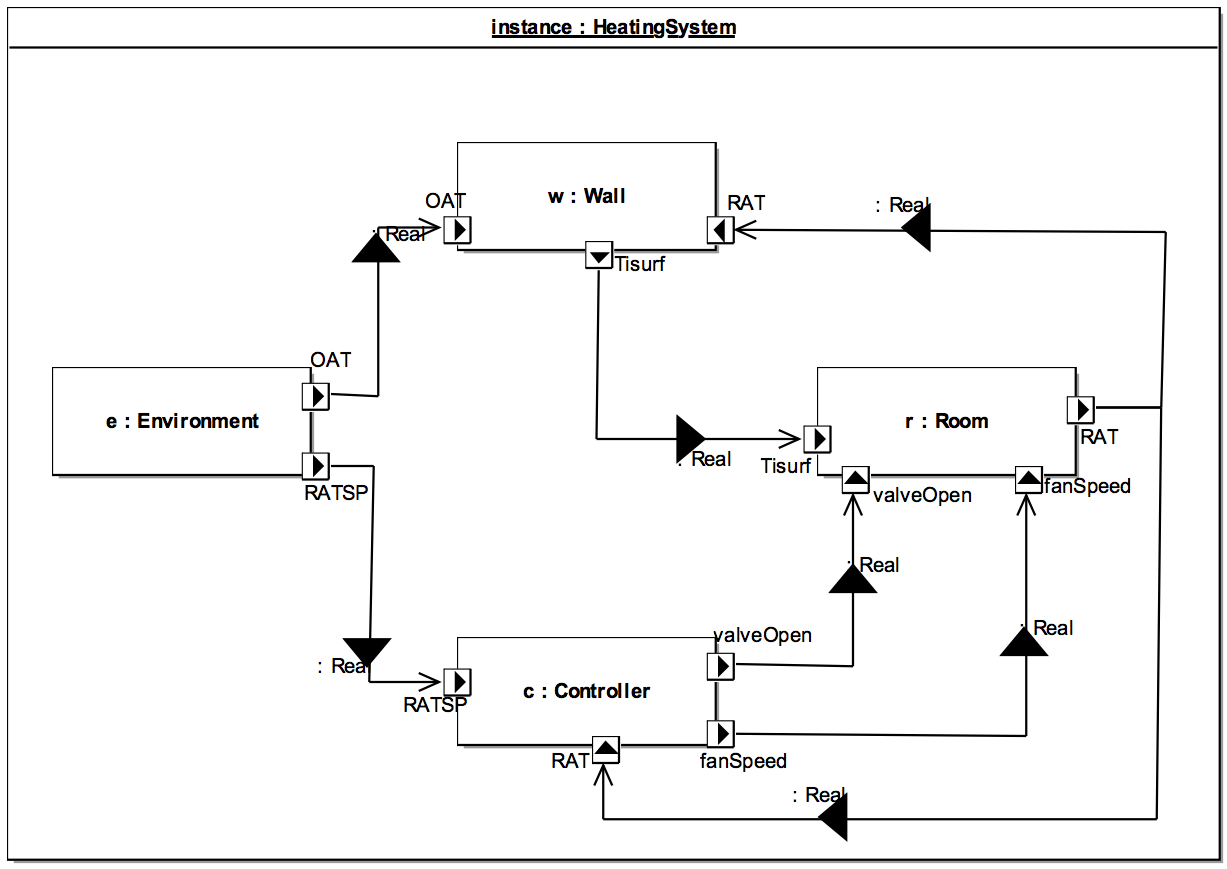
\includegraphics[width=0.7\linewidth]{fcu/fcu_sysml_cd_mm}
%     \caption{SysML Connection Diagram using INTO-CPS profile corresponding to the `pure' multi-model approach}
%     \label{fig:fcu_sysml_mm_cd}
%  \end{center}
%\end{figure}

\subsection{Multi-model}
\label{sec:fcu_into_mm}

\subsubsection{Models}
\label{sec:fcu_into_models}

%Given the constituent elements identified in the SysML models above, the FCU pilot study comprises several (simulation) models for the 3- and 4-version of the pilots.
%
%\subsubsection*{Models -- 3-model version}

%The 3-model version 
This pilot 
comprises two 20-sim models: \texttt{RoomHeating} and the \texttt{Environment}; an OpenModelica \texttt{RoomHeating\_OM} model; and a \texttt{Controller} VDM-RT model. %Figure~\ref{fig:fcu_20-sim-RH_mm} depicts a 20-sim model with two blocks used to generate the \emph{RoomHeating} and \emph{Environment} FMUs. 

\begin{description}
  \item[RoomHeating.emx] Figure~\ref{fig:fcu_20-sim-RH_rg} shows the \emph{RoomHeating} subsystem with blocks for the room and the wall. The model takes inputs for the required room temperature, outside air temperature, fan speed and valve control. The model outputs the current room air temperature. 
 
\begin{figure}[htb!]
  \begin{center}
     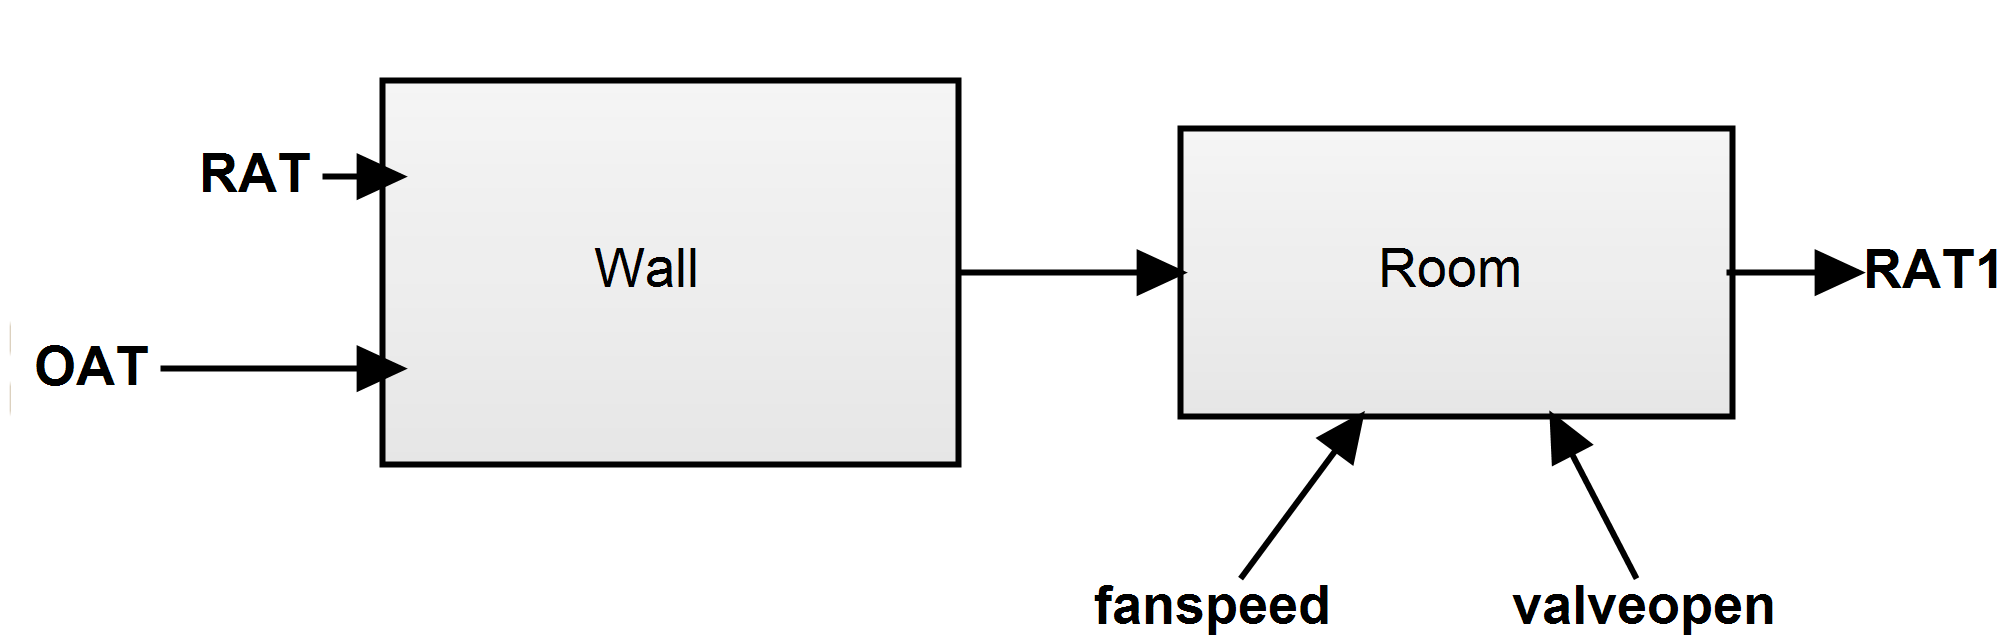
\includegraphics[width=0.6\linewidth]{fcu/fcu_rh} 
     \caption{RoomHeating model}
      \label{fig:fcu_20-sim-RH_rg}
  \end{center}
\end{figure}

\item[RoomHeating\_OM.mo] The OpenModelica version of the \emph{RoomHeating} subsystem is similar to that of the 20-sim version -- it also comprises blocks for the room and wall, with the same interface. The block diagram is shown in Figure~\ref{fig:fcu_om-RH_rg}.
 
\begin{figure}[htb!]
  \begin{center}
     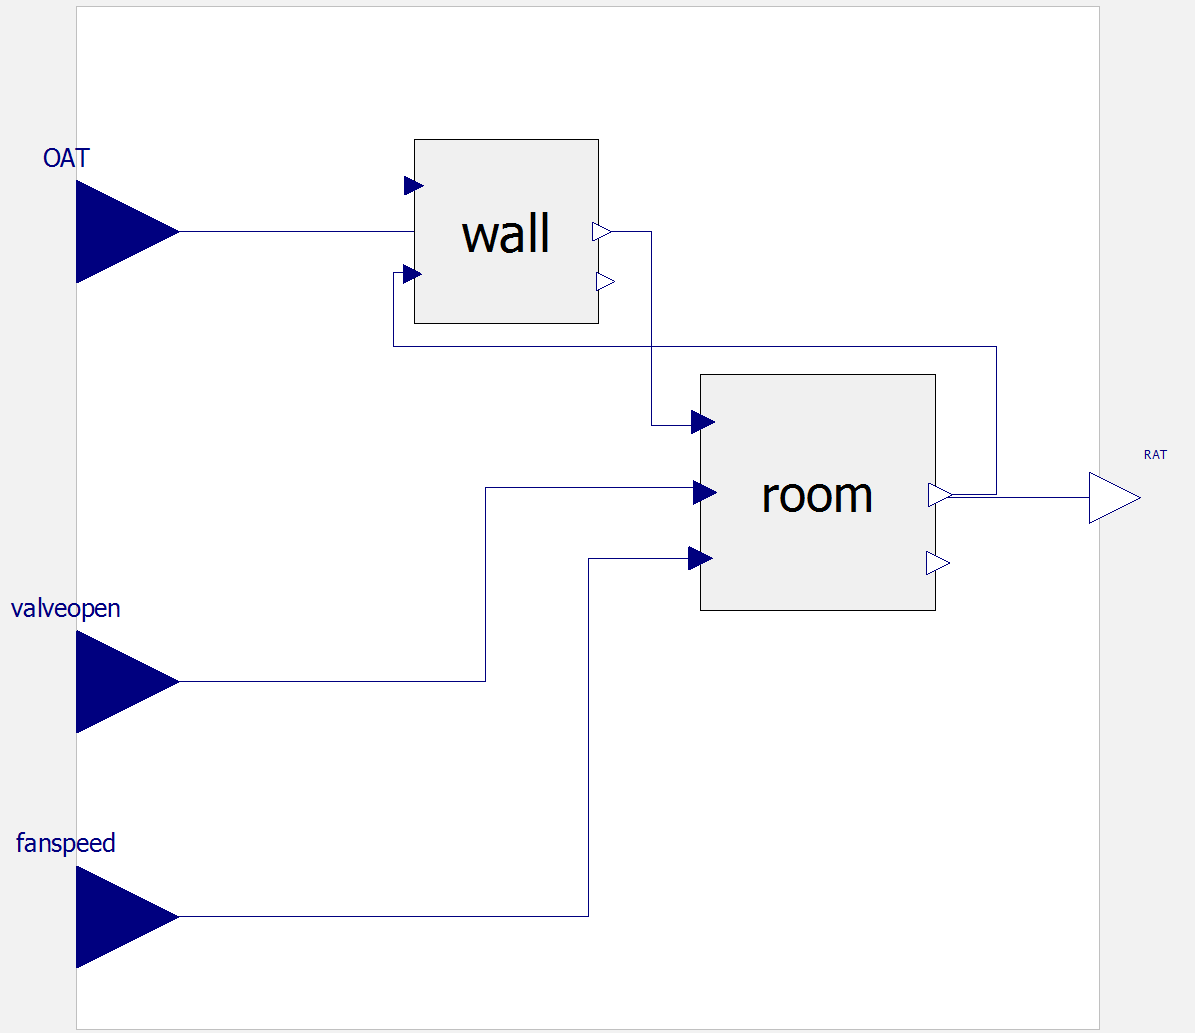
\includegraphics[width=0.6\linewidth]{fcu/fcu_rh_om} 
     \caption{RoomHeating model}
      \label{fig:fcu_om-RH_rg}
  \end{center}
\end{figure}


  \item[Environment.emx] The \emph{Environment} model, in Figure~\ref{fig:fcu_20-sim-RH_e}, provides data on the environment outside air temperature and scenario data based on change of room temperature set point.
  
\begin{figure}[htb!]
  \begin{center}
   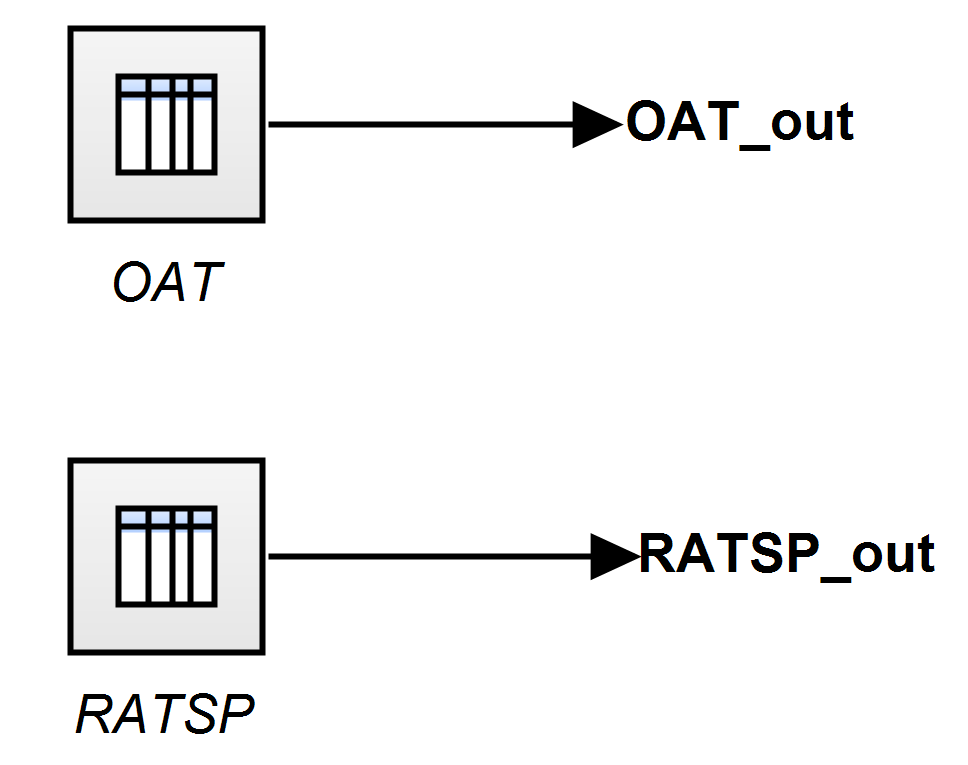
\includegraphics[width=0.35\linewidth]{fcu/fcu_env} 
     \caption{Environment model}
     \label{fig:fcu_20-sim-RH_e}
  \end{center}
\end{figure}

  \item[ControllerFCU] The VDM controller model comprises a \emph{Sensor} class, which provides access to the current room temperature, and a \emph{LimitedActuator} class, which provides output for the valveOpen and fanSpeed values. The actuator is limited such that values fall only between the real values 1.0 and 0.0000001.
\end{description}

%\subsubsection*{Models -- 4-model version}
%
%The 4-model version shares the \texttt{Environment} and \texttt{Controller} with the previous multi-model, 
%splitting the \texttt{RoomHeating} model into separate \texttt{Room} and \texttt{Wall} models. %This is shown in Figure~\ref{fig:fcu_20-sim-RH_mm4},
%
%\begin{description}
%  \item[Room] The \emph{Room} model, shown in Figure~\ref{fig:fcu_20-sim-RH_r}, consists of a single block containing 
%a collection of equations to determine the room air temperature (\emph{RAT}) based upon the temperature of the walls and the FCU fan and valve values.
%      
%\begin{figure}[htb!]
%  \begin{center}
%      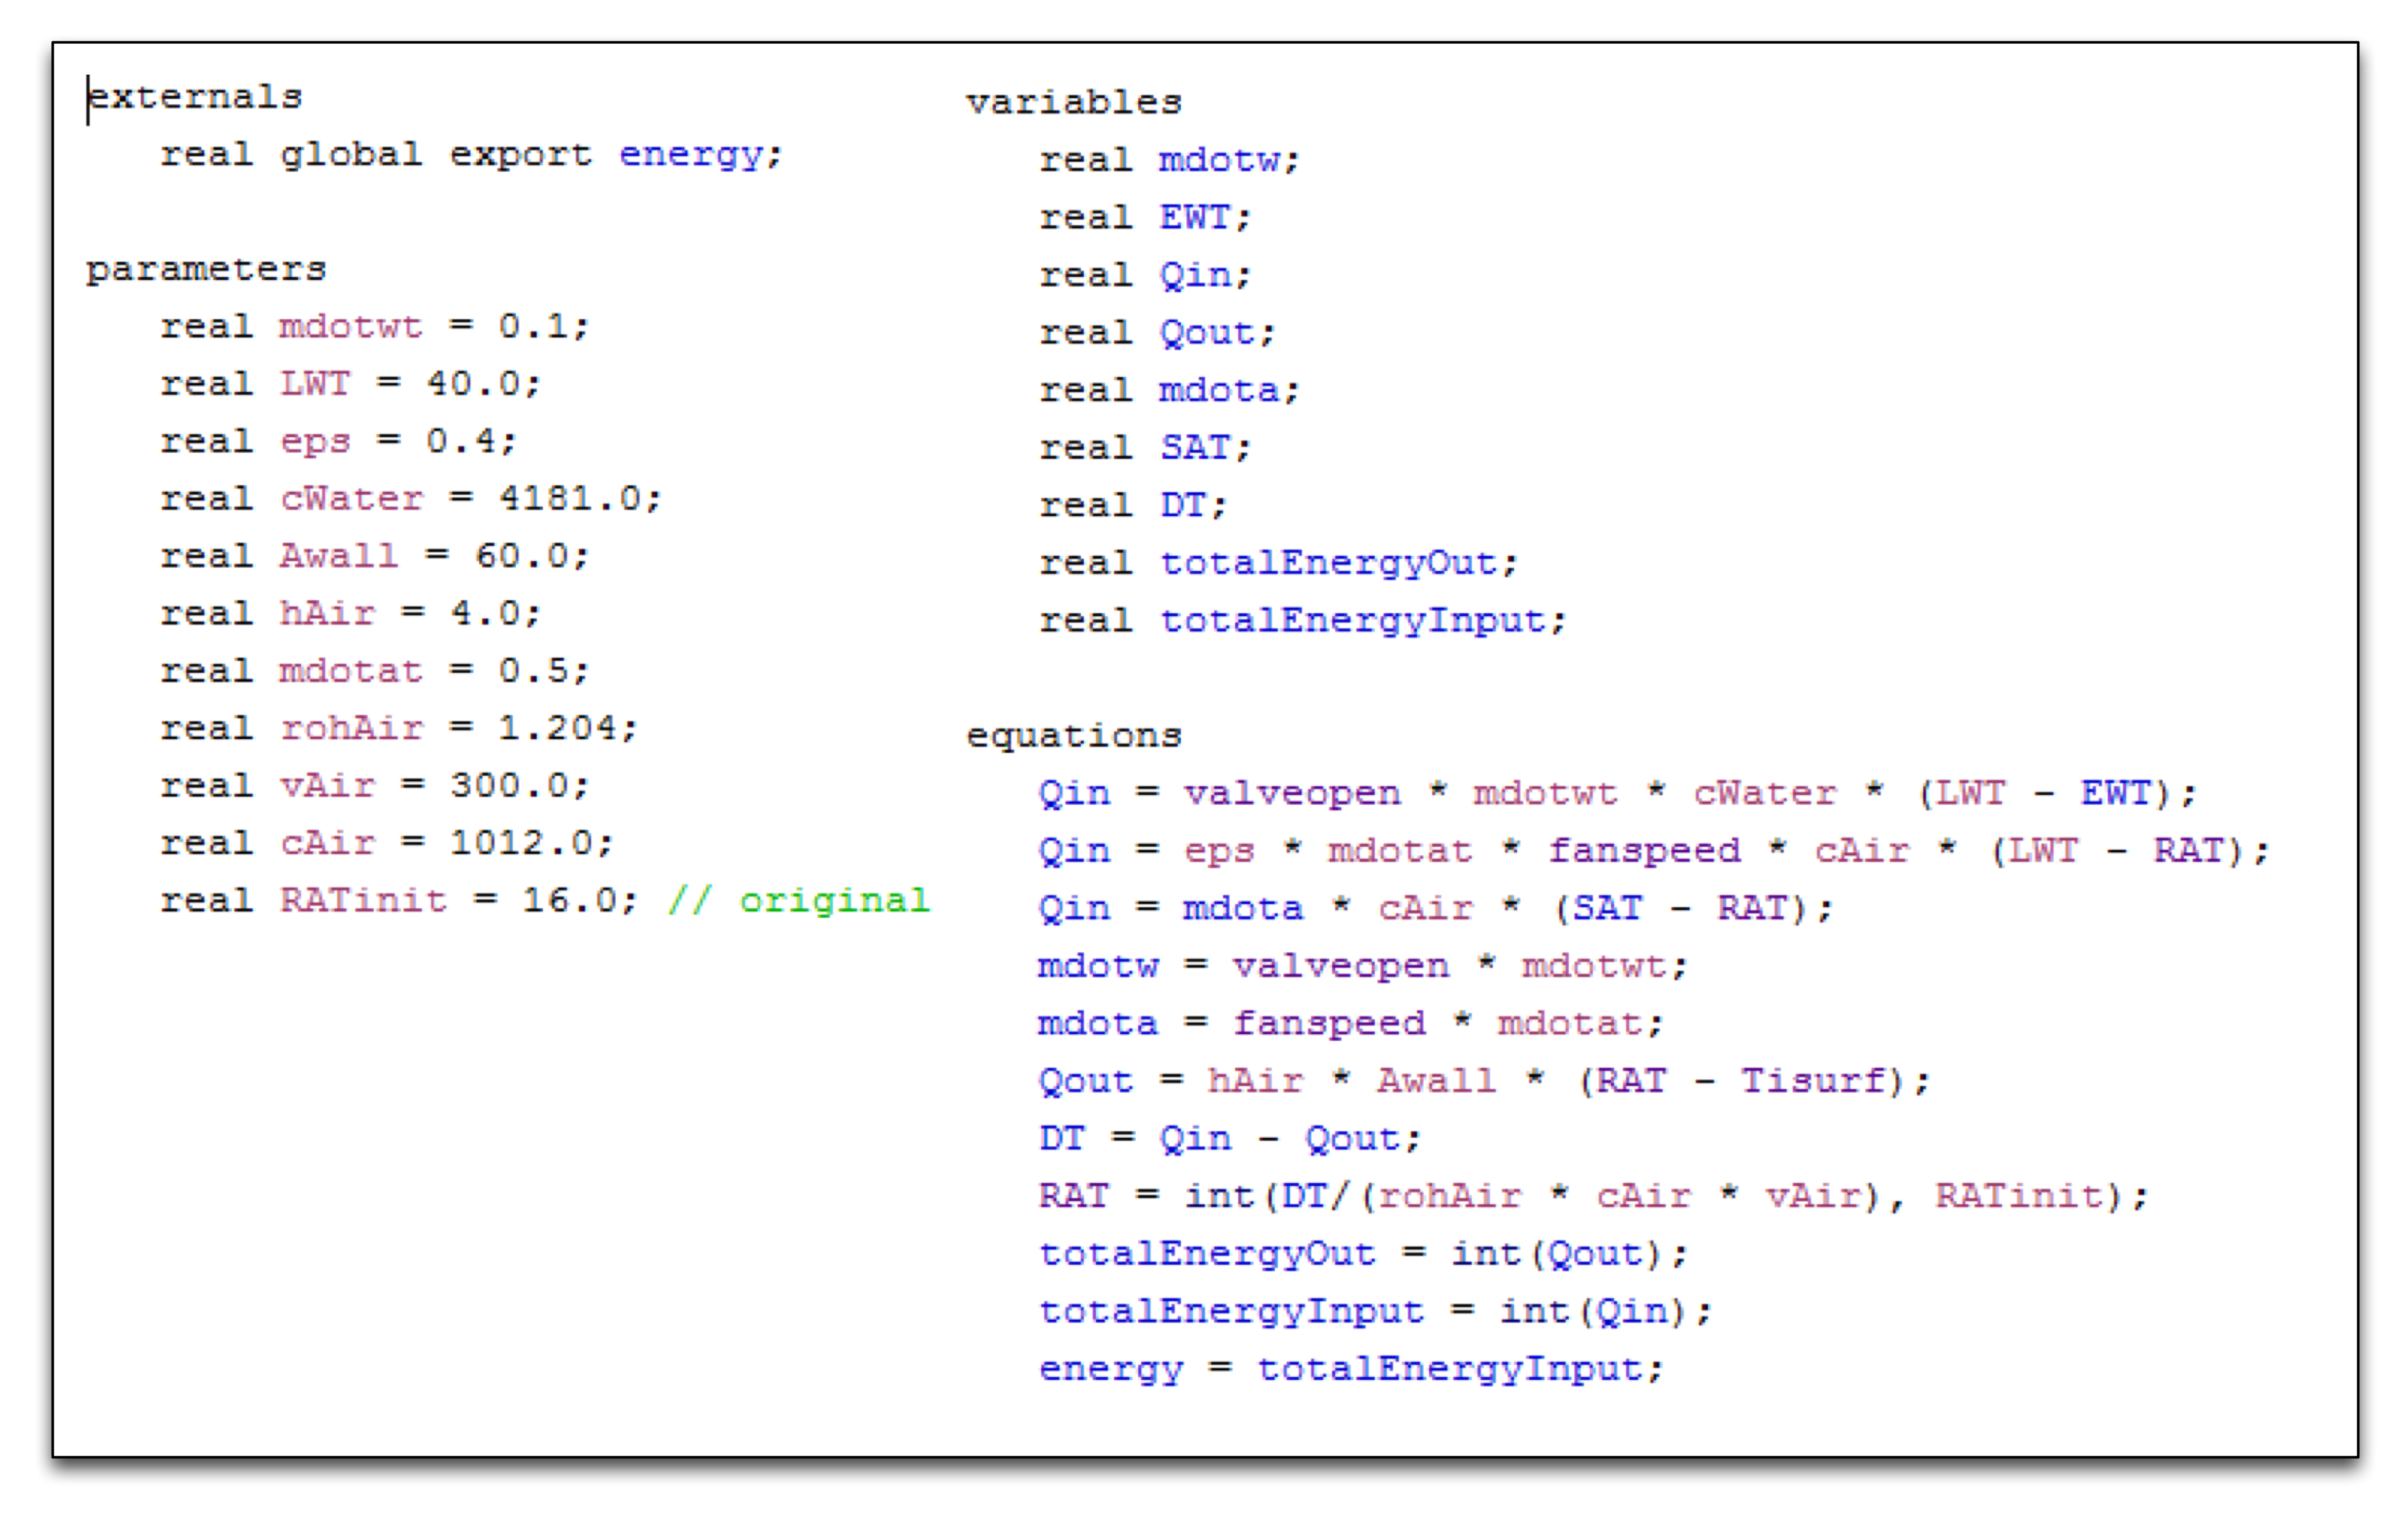
\includegraphics[width=0.8\linewidth]{fcu/fcu_room} 
%     \caption{Room model}
%      \label{fig:fcu_20-sim-RH_r}
%  \end{center}
%\end{figure}
%
%  \item[Wall] The \emph{Wall} model, in Figure~\ref{fig:fcu_20-sim-RH_w}, is again represented by a single block. Two design parameters allow designers to vary the  thermal conductivity and density. Based upon properties of the wall, the model outputs the surface air temperature (\emph{Tisurf}) given the outside room temperature and inside room air temperature. 
%  
%\begin{figure}[htb!]
%  \begin{center}
%   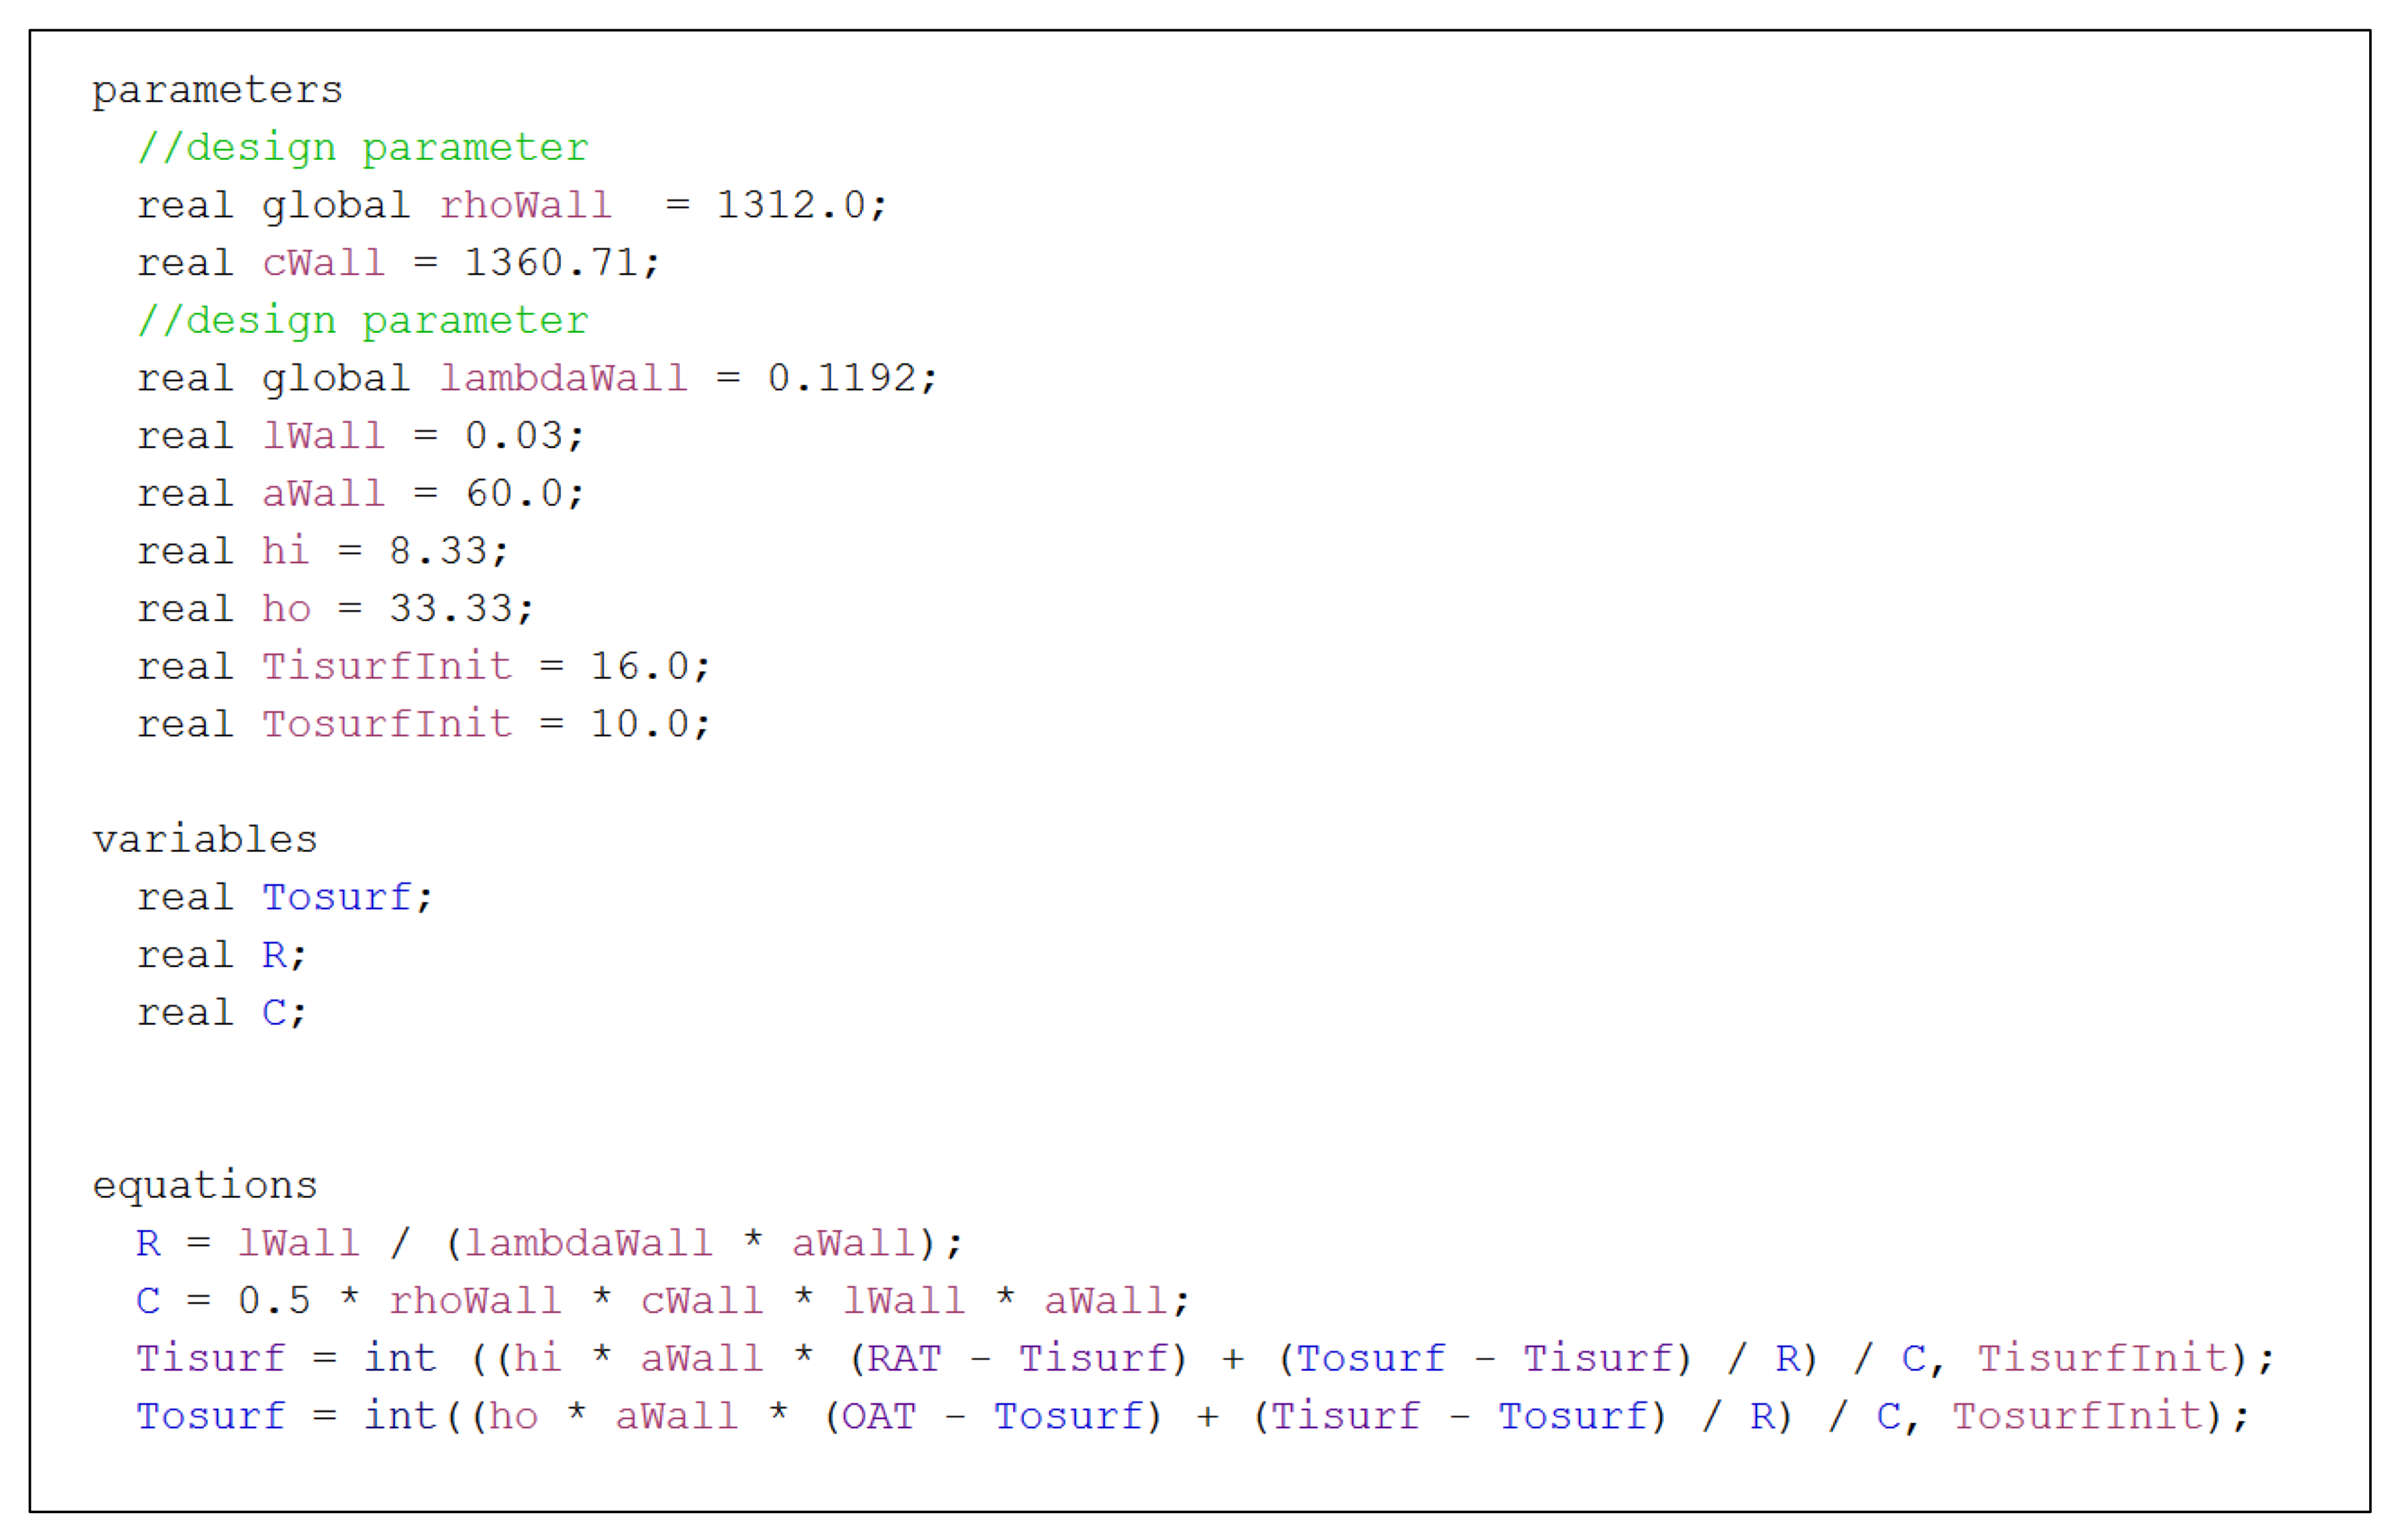
\includegraphics[width=0.9\linewidth]{fcu/fcu_wall} 
%     \caption{Wall model}
%      \label{fig:fcu_20-sim-RH_w}
%  \end{center}
%\end{figure}
%  
%  \item[Environment] This is unchanged from the 3-model version.
%  \item[Controller] This is unchanged from the 3-model version.
%\end{description}

% It is worth re-iterating that the \emph{Room} and \emph{Wall} blocks are composed in the 3-model \emph{RoomHeating} block.


\subsubsection{Configuration}
\label{sec:fcu_into_conf}

%\subsubsection*{3-model version}
%
The multi-model comprises three FMUs and five connections. The FMUs -- \texttt{FCUController.fmu}, \texttt{RoomHeating.fmu} and \texttt{Environment.fmu} -- are exported from the VDM-RT and 20-sim models.  

The connections are as follows: 
\begin{itemize}
\item from the \emph{EnvironmentFMUs} \texttt{RAT\_OUT} port to the \emph{ControllerFMU} \texttt{RATSP} port;
\item from the \emph{EnvironmentFMUs} \texttt{OAT\_OUT} port to the \emph{RoomHeatingFMU} \texttt{OAT} port;
\item from the \emph{ControllerFMUs} \texttt{valveOpen} port to the \emph{RoomHeatingFMU} \texttt{valveopen} port;
\item from the \emph{ControllerFMUs} \texttt{fanSpeed} port to the \emph{RoomHeatingFMU} \texttt{fanspeed} port; and
\item from the \emph{RoomHeatingFMU} \texttt{RAT} port to the \emph{ControllerFMUs} \texttt{RAT} port.
\end{itemize}

%There are no parameters to set.
%
%\subsubsection*{4-model version}
%
%In the 4-model version of the FCU multi-model there are 4 FMUs and 7 connections. The 4 FMUs -- \texttt{FCUController.fmu}, \texttt{Room.fmu}, \texttt{Wall.fmu} and \texttt{Environment.fmu} -- are exported from the VDM-RT and 20-sim models.  
%
%The connections are as follows: 
%\begin{itemize}
%\item from the \emph{EnvironmentFMUs} \texttt{RAT\_OUT} port to the \emph{ControllerFMU} \texttt{RATSP} port;
%\item from the \emph{EnvironmentFMUs} \texttt{OAT\_OUT} port to the \emph{WallFMU} \texttt{OAT} port;
%\item from the \emph{WallFMU} \texttt{Tisurf} port to the \emph{RoomFMUs} \texttt{Tisurf} port;
%\item from the \emph{RoomFMU} \texttt{RAT} port to the \emph{WallFMUs} \texttt{RAT} port;
%\item from the \emph{RoomFMU} \texttt{RAT} port to the \emph{ControllerFMUs} \texttt{RAT} port;
%\item from the \emph{RoomFMU} \texttt{energy} port to the \emph{ControllerFMUs} \texttt{energyIn} port;
%\item from the \emph{ControllerFMUs} \texttt{valveOpen} port to the \emph{RoomFMU} \texttt{valveopen} port; and
%\item from the \emph{ControllerFMUs} \texttt{fanSpeed} port to the \emph{RoomFMU} \texttt{fanspeed} port.
%\end{itemize}

There are three parameters to set: \emph{lambdaWall} and \emph{rhoWall} which define the \texttt{Wall} thermal conductivity and density respectively, and \emph{controllerFrequency}, which defines the frequency of the \texttt{Controller}. The standard parameters for these are $1.1192$, $1312$ and $1000000000$ respectively. These may be adjusted for the purposes of DSE.

\subsection{Co-simulation}
\label{sec:fcu_into_co}

Co-simulation of the full scenario (outside air temperature and room set point) has a duration of 6800 seconds. Running the two multi-models produces the same results. The results as displayed in the INTO-CPS application are shown in Figure~\ref{fig:fcu_results}, and values of note sent between FMUs are shown separately in Figure~\ref{fig:fcu_results2}.

\begin{figure}[htb!]
\begin{center}
   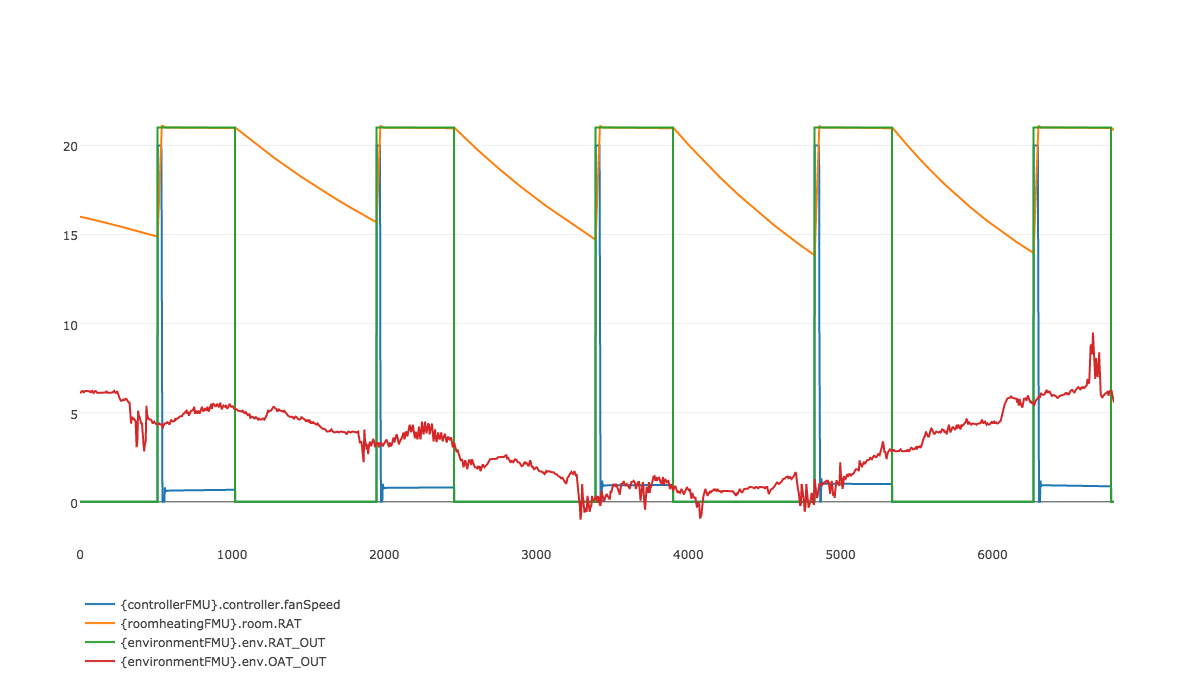
\includegraphics[width=1\linewidth]{fcu/fcu_cosim_app} 
  \caption{Co-simulation results as shown in lNTO-CPS application live stream}
\label{fig:fcu_results}
\end{center}
\end{figure}

\begin{figure}[htb!]
\begin{center}
   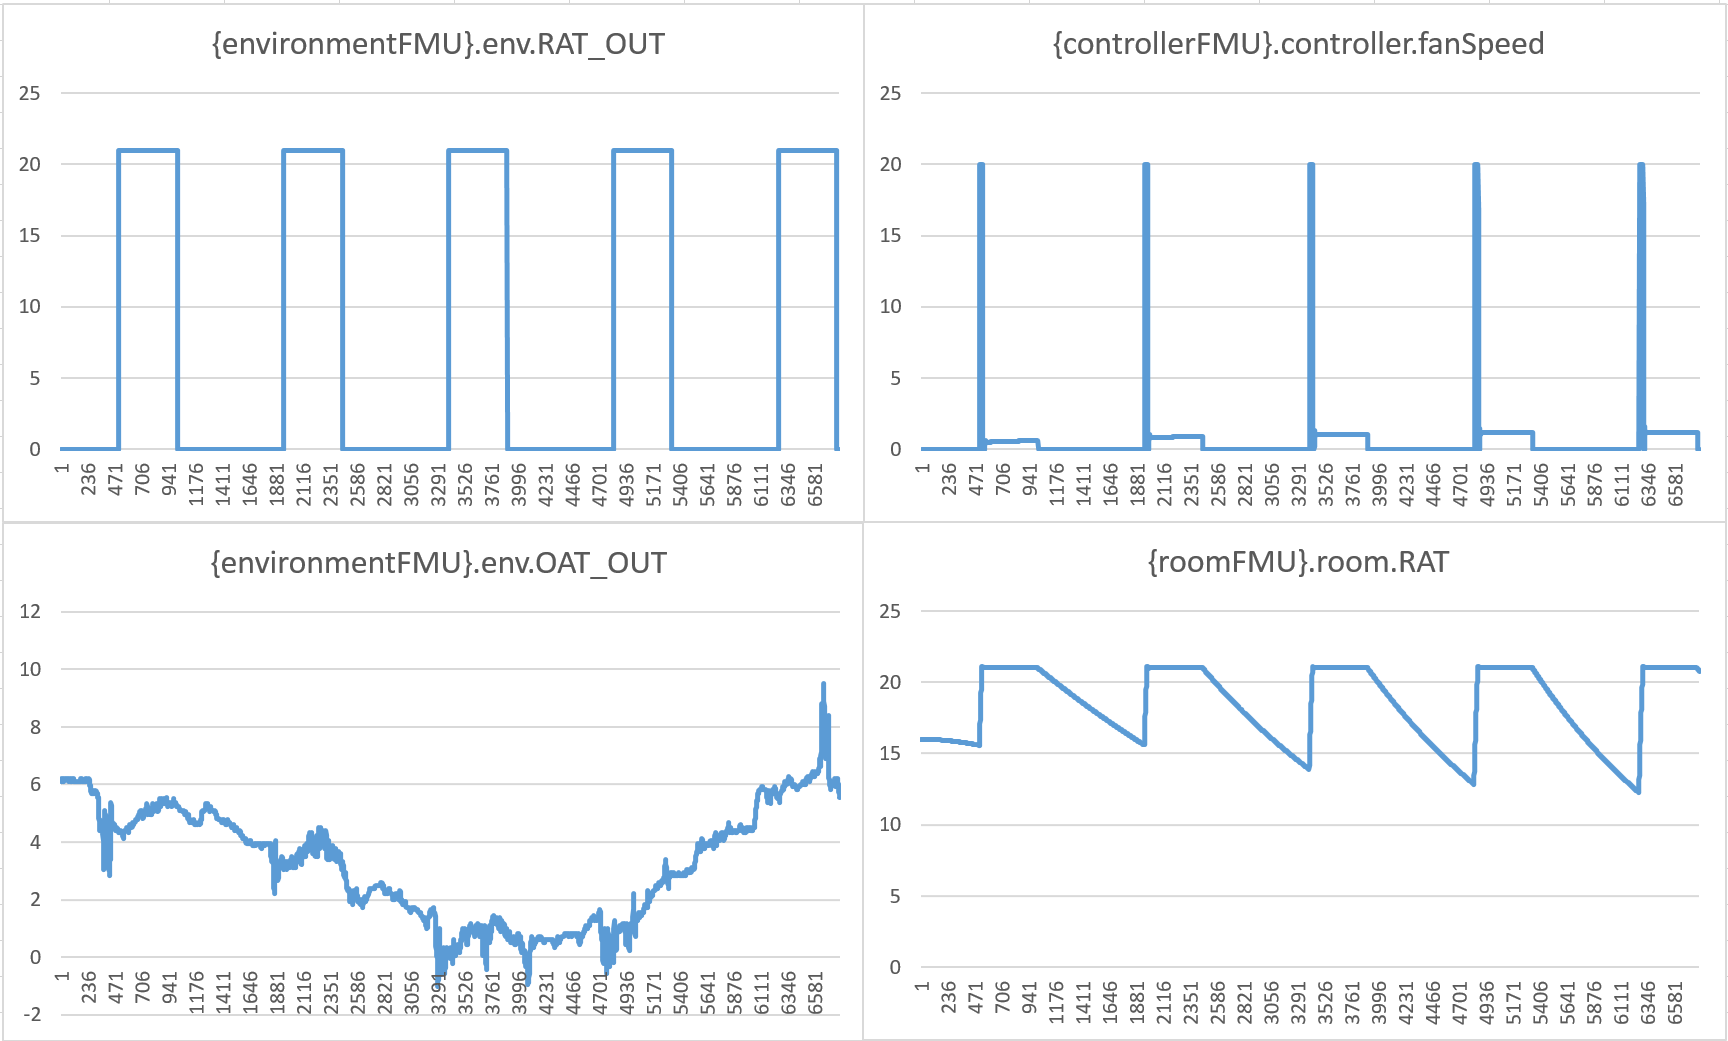
\includegraphics[width=1\linewidth]{fcu/fcu_results} 
  \caption{Co-simulation results as shown in graphs from result log files}
\label{fig:fcu_results2}
\end{center}
\end{figure}

The results in Figure~\ref{fig:fcu_results2} show that the set point (top left) is toggled between 20 and 0, with the fan (and valve) are adjusted to achieve the set point. The bottom right graph shows the ultimate result of the simulation -- that the Room Air Temperature (RAT) meets the set point, maintains that temperature whilst required and then slowly drop in temperature until the set point returns to 20.

As mentioned in Section~\ref{sec:fcu_into_conf}, the  \emph{lambda\_Wall}, \emph{rhoWall} and \emph{controllerFrequency} design parameters may be altered to test different wall properties and their effect on the overall CPS.

\subsection{Analyses and Experiments}
\label{sec:fcu_analyses}

\subsubsection{Design Space Exploration}
\label{sec:fcu_dse}

Detailed in Section~\ref{sec:fcu_into_conf}, the multi-model has three design parameters, \emph{lambda\_Wall}, \emph{rhoWall} and \emph{controllerFrequency} which define the wall thermal conductivity, wall density and controller frequency respectively, which may be altered to perform DSE. 

This example has 2 DSE experiments:

\begin{description}
\item [fcu-walls:] The parameter values for \emph{lambda\_Wall} ranges from $0.1192$ to $10.1192$ in intervals of $0.25$, and the \emph{rhoWall} value may be either $1312.0$ or $1400.0$. In this experiment a wide range of \emph{lambda\_Wall} values (40 in total) provides a 80-model design space -- no constraints are defined. Two objectives are defined, using internal DSE functions, \emph{energyConsumed} and \emph{averageTemperature}. The first objective is to retrieve the maximum energy usage value, this is essentially the final value of the energy port. The second is to return the mean RAT -- that  is the average temperature of the RAT, which shows how the room heats and cools over time depending upon the different wall values. 

The Pareto ranking seeks to maximise the average temperature and minimise the energy consumed. Figure~\ref{fig:fcu_dse1} shows that there is one experiment at rank 1 (the green dot), which indicates that (as is intuitive) the best design is that with the lowest thermal conductivity and greater density. 

\begin{figure}[htb!]
\begin{center}
   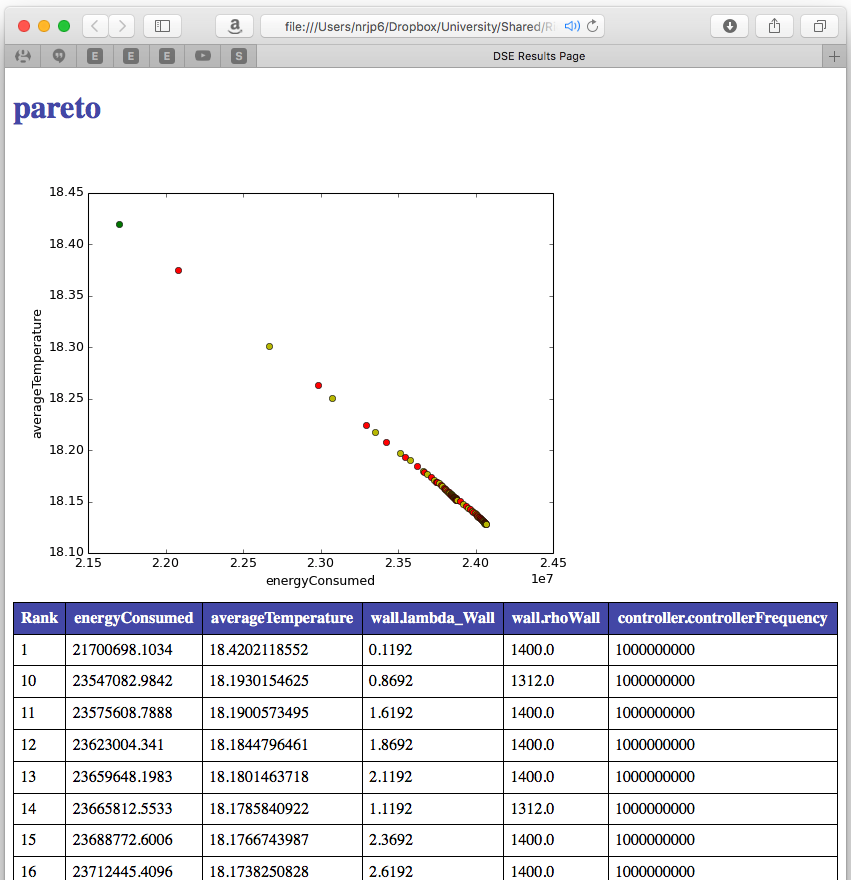
\includegraphics[width=1\linewidth]{fcu/fcu-dse1} 
  \caption{DSE results for \textbf{fcu-walls} experiment}
\label{fig:fcu_dse1}
\end{center}
\end{figure}

\item [fcu-walls-controller:] The second experiment varies the \emph{lambda\_Wall} and \emph{rhoWall} as earlier, but with a different collection of values: \emph{lambda\_Wall} ranges from $0.1192$ to $10.1192$ in intervals of $1.0$, and the \emph{rhoWall} value ranging from $1300.0$ to $1700.0$ in intervals of $1000.0$. In addition, the  \emph{controllerFrequency} parameter is varied between $800000000$ and $1200000000$ in intervals of $100000000$. A  space of 250 designs is defined. The same objectives and rankings are used as the above DSE experiment.

Figure~\ref{fig:fcu_dse2} shows that there are five experiments at rank 1 (the green dots), which indicates that (as is intuitive) the best design is that with the lowest thermal conductivity and greater density, with the controller frequency providing only marginal impact. It is interesting to note that the frequency does have an impact on both the   \emph{energyConsumed} and \emph{averageTemperature} objectives.

\begin{figure}[htb!]
\begin{center}
   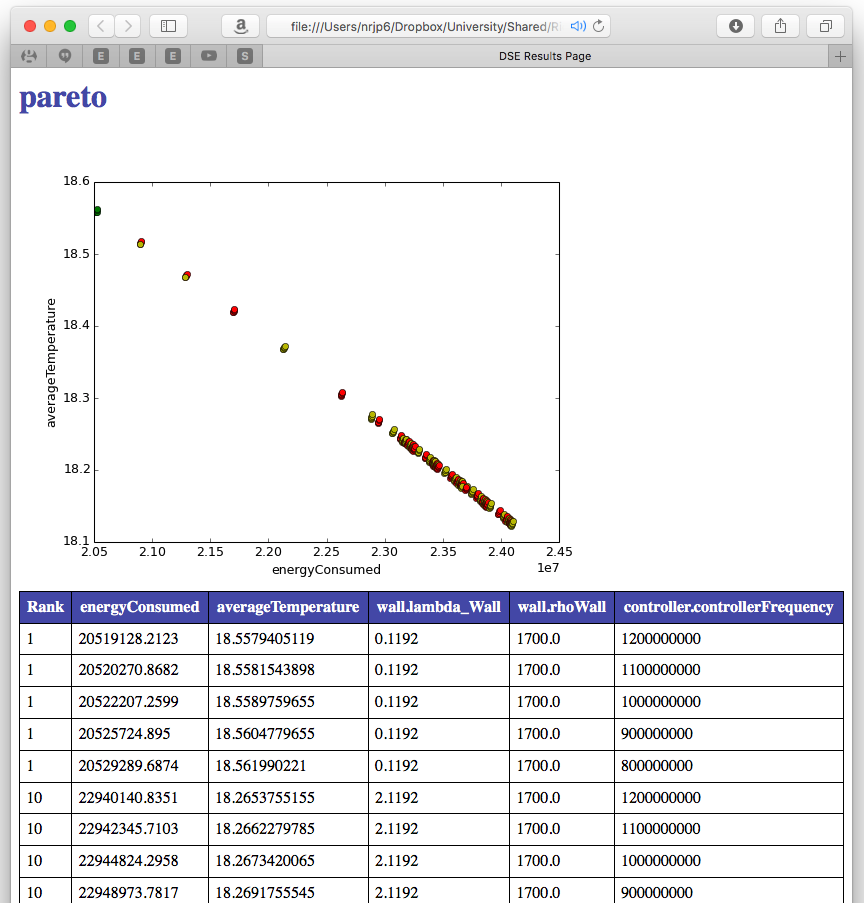
\includegraphics[width=1\linewidth]{fcu/fcu-dse2} 
  \caption{DSE results for \textbf{fcu-walls-controller} experiment}
\label{fig:fcu_dse2}
\end{center}
\end{figure}



\end{description}

\subsubsection{Test Automation and Model Checking}
\label{sec:fcu_ta}
\graphicspath{ {./fcu/TA/} }
In this pilot study, test automation is applied to the system, including not only the discrete FCU controller but also the continuous room and wall. A test model in SysML models both discrete and continuous parts together. Accordingly, we developed two SUT implementations that have different scope. The first SUT has a controller implemented in C, and uses two 20-Sim models for the \emph{Room} and the \emph{Wall} separately. While the second SUT has all (the \emph{Controller}, \emph{Wall} and \emph{Room}) implemented in C in the same program. With the two SUTs and an additional SUT called \T{Simulation} that is automatically generated from the test model in RT-Tester, we can construct three test automation configurations. And each configuration corresponds to one SUT.

Subsequently, we present the test model in SysML, then the two SUT implementations, and finally test results for three different configurations.

\paragraph{Test Model}
The developed test model consists of a \emph{Controller}, a \emph{Room} model, and a \emph{Wall} model. We use the Euler method to model continuous parts \emph{Wall} and \emph{Room}. 

Similar to the test model for \emph{Three-tank Water Tank} in Section~\ref{sec:threetank_ta}, the SysML model consists a SUT and a TE. They are represented by the blocks \emph{SystemUnderTest} and \emph{TestEnvironment}. Both of them have two ports with \emph{Observables} and \emph{Stimuli} interfaces respectively. From the SUT perspective, the port of
\emph{Observables} is an output port, and the port of \emph{Stimuli} is an input port. However, their corresponding ports in the TE are in the opposite direction. For brevity, we omit the ASD and CD diagrams of the \emph{System} in this document.

\subparagraph{Inputs and Outputs}
The \emph{SystemUnderTest} receives the following inputs (stimuli) from the \emph{TestEnvironment}:
\begin{itemize}
    \item $OAT$: Outside Air Temperature;
    \item $RATSP$: Room Air Temperature Set Point.
\end{itemize}

The \emph{SystemUnderTest} provides the following observable outputs to the \emph{TestEnvironment}:
\begin{itemize}
    \item $RAT\_out$: Room Air Temperature.
\end{itemize}

\subparagraph{SystemUnderTest}
The \emph{SystemUnderTest} consists of a FCU controller, a wall model, and a room model.

The architecture structure diagram of \emph{SystemUnderTest} is shown in Figure~\ref{fig:fcu_sut_sad}. 
\begin{figure}[htb!]
    \centering
	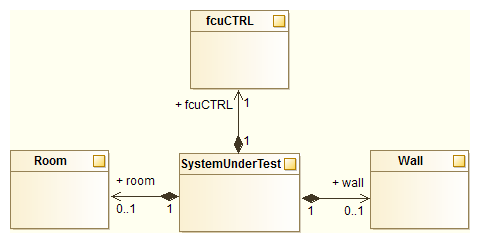
\includegraphics[width=0.8\textwidth]{roomwall/fcu_sut_sad}
    \caption{Architecture Structure Diagram of SUT}
    \label{fig:fcu_sut_sad}
\end{figure}

\subparagraph{FCU Controller}
The \emph{fcuCTRL} receives the following inputs (stimuli):
\begin{itemize}
    \item $RAT\_out$: Room Air Temperature from the \emph{Room};
    \item $RATSP$: Room Air Temperature Set Point from the \emph{TestEnvironment}.
\end{itemize}

The \emph{fcuCTRL} provides the following outputs to the \emph{Room}:
\begin{itemize}
    \item $fanSpeed$: Fan Speed; 
    \item $valveOpen$: Valve Open State.
\end{itemize}

The state machine diagram of the \emph{fcuCTRL} is illustrated in Figure~\ref{fig:fcu_sut_fcuctrl_sm}.
\begin{figure}[htb!]
    \centering
	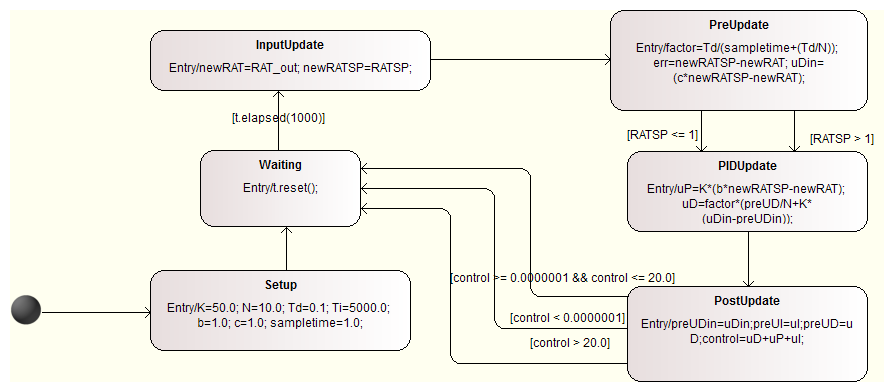
\includegraphics[width=1.0\textwidth]{roomwall/fcu_sut_fcuctrl_sm}
    \caption{State Machine Diagram of fcuCTRL}
    \label{fig:fcu_sut_fcuctrl_sm}
\end{figure}

In the diagram,
\begin{itemize}
    \item \T{Setup} is used to initialize constant variables;
    \item After \T{Setup}, the state machine resides in the \T{Waiting} state, most of the time;
    \item Then every second, it starts to calculate PID parameters again:
        \begin{itemize}
            \item At first, the inputs $RAT$ and $RATSP$ are copied to local variables to make sure all subsequent computations refer to same values of $RAT$ and $RATSP$;
            \item Then, $uP$, $uD$, $uI$, and other local variables are computed for future use,
            \item Next, the summation of $uP$, $uD$, and $uI$ is calculated and assigned to $control$,
            \item Finally, we limit $control$ and assign it to $fanSpeed$ and $valveSpeed$ respectively in the transitions from \T{PostUpdate} to \T{Waiting}.
        \end{itemize}
\end{itemize}

\subparagraph{Wall}
The \emph{Wall} receives the following inputs (stimuli):
\begin{itemize}
    \item $RAT\_out$: Room Air Temperature from the \emph{Room}; 
    \item $OAT$: Outside Air Temperature from the \emph{TestEnvironment}.
\end{itemize}

And the \emph{Wall} provides the following outputs to \emph{Room}:
\begin{itemize}
	\item $Tisurf$: Wall Internal Surface Temperature.
\end{itemize}

The state machine diagram of the \emph{Wall} is illustrated in Figure~\ref{fig:fcu_sut_wall_sm}.
\begin{figure}[htb!]
    \centering
	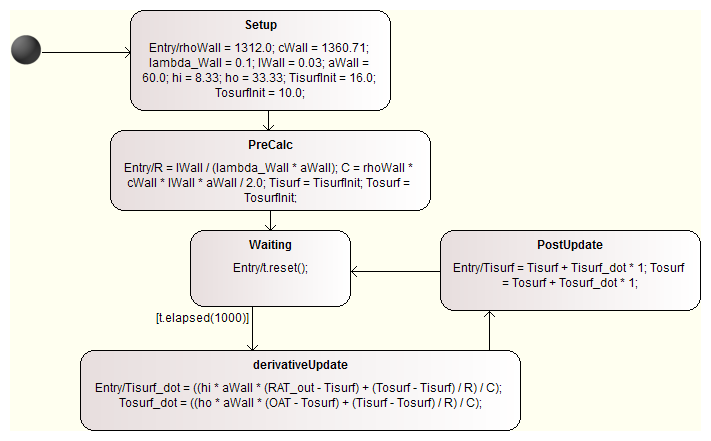
\includegraphics[width=1.0\textwidth]{roomwall/fcu_sut_wall_sm}
    \caption{State Machine Diagram of Wall}
    \label{fig:fcu_sut_wall_sm}
\end{figure}

In the diagram,
\begin{itemize}
    \item \T{Setup} is used to initialize constant variables;
    \item After \T{Setup}, we calculate the constants $R$ and $C$, and initialize $Tisurf$ and $Tosurf$ in \T{PreCalc} according to other constants that are initialized in \T{Setup}. 
    \item Then the state machine resides in the \T{Waiting} state, most of the time. And every second, it starts to calculate and update $Tisurf$ and $Tosurf$ again:
        \begin{itemize}
            \item The derivatives of $Tisurf$ and $Tosurf$ are calculated in \T{derivativeUpdate}, 
            \item Then, they are used in \T{PostUpdate} to update $Tisurf$ and $Tosurf$ according to the Euler Methods. 
        \end{itemize}
\end{itemize}

\subparagraph{Room}
The \emph{Room} receives the following inputs (stimuli):
\begin{itemize}
    \item $fanSpeed$: Fan Speed from the \emph{fcuCTRL};
    \item $valveOpen$: Valve Open State from the \emph{fcuCTRL};
    \item $Tisurf$: Wall Internal Surface Temperature from the \emph{Wall}.
\end{itemize}

The \emph{Room} provides the following outputs to the \emph{fcuCTRL} and \emph{TestEnvironment}:
\begin{itemize}
    \item $RAT\_out$: Room Air Temperature.
\end{itemize}

The state machine diagram of the \emph{Room} is illustrated in Figure~\ref{fig:fcu_sut_room_sm}.
\begin{figure}[htb!]
    \centering
	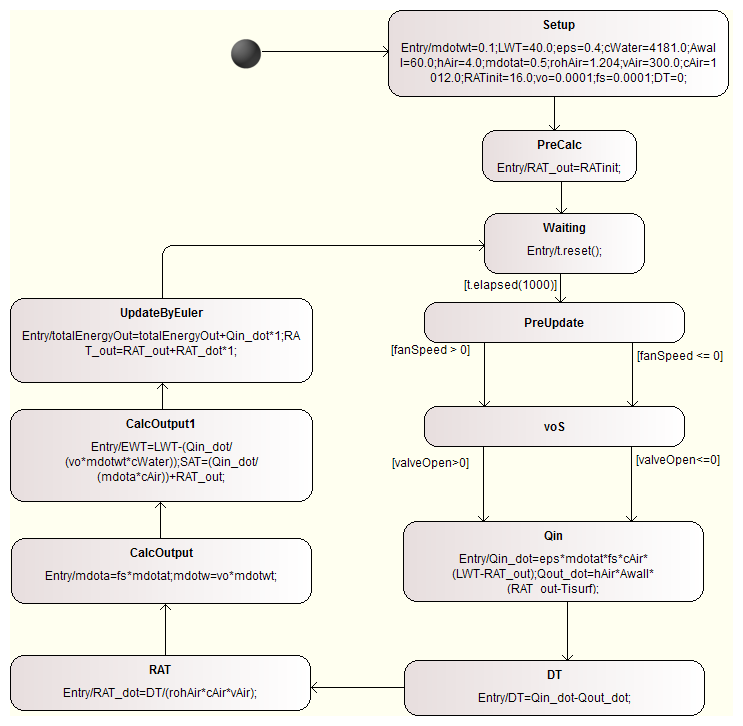
\includegraphics[width=1.0\textwidth]{roomwall/fcu_sut_room_sm}
    \caption{State Machine Diagram of Room}
    \label{fig:fcu_sut_room_sm}
\end{figure}

In the diagram,
\begin{itemize}
    \item Similarly, \T{Setup} is used to initialize constant variables;
    \item After \T{Setup}, we set $RAT\_out$ to $RATinit$ in \T{PreCalc}. 
    \item Then the state machine resides in the \T{Waiting} state, most of the time. And every second, it starts to calculate and update $RAT\_out$:
        \begin{itemize}
            \item Validality of the inputs $fanSpeed$ and $valveOpen$ are checked at first,
            \item Then, the derivatives of $Qin$ (heat transferred to the air in the coil) and $Qout$ (heat lost through room and walls) are calculated,
            \item Subsequently, the derivative of $RAT$ is calculated, and intermediate $SAT$ (supply air temperature) and $EWT$ (entering water temperature) are updated as well.
            \item In the end, the output $RAT\_out$ is updated by the Euler method.
        \end{itemize}
\end{itemize}

\subparagraph{Test Input Simulation} The automatically generated test cases from a test model using RTT-MBT in RT-Tester is hardly realistic for a real life scenario. In order to provide reasonable inputs to Co-simulation, we use a real input sequence for $OAT$ and $RATSP$ in \T{Multi-models}. However, it is not possible for RTT-MBT to give this as input since RTT-MBT uses a SMT solver to generate test cases, or uses a state machine to specify the input sequence in \T{TestEnvironment} of the test model. 
We use the second way to specify the input sequence by defining a state machine in a block \T{TESim} of \T{TestEnvironment}. The diagram is shown in Figure~\ref{fig:fcu_co_te_sim}. The specified sequence is shown as $SUT\_OAT$ and $SUT\_RATSP$ in Figure~\ref{fig:fcu_co-sim-result}. Basically, $OAT$ changes slightly but $RATSP$ vibrates between 10 and 35 \textdegree{}C.
\begin{figure}[htb!]
    \centering
	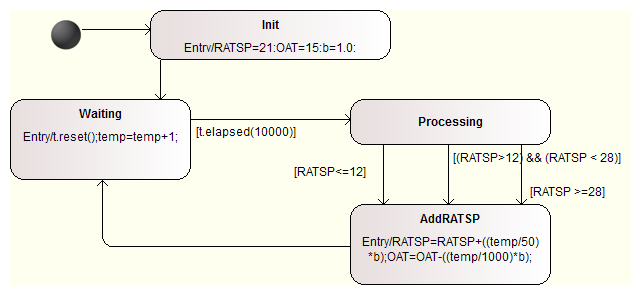
\includegraphics[width=0.8\textwidth]{tesim}
    \caption{State machine diagram of TESim}
    \label{fig:fcu_co_te_sim}
\end{figure}

\paragraph{Manual Implementations of SUT}
Two SUTs are implemented. The first one is a SUT with the \emph{Controller} in C, and then reuses the \emph{Wall} and \emph{Room} models in 20-Sim or Modelica. And the second one is a standalone C program which has all three parts together. By using a Python script named ``build-suts.py'', we can build, assemble, and wrap them into FMUs in RT-Tester automatically. The corresponding FMU for the first implementation is named \T{SUT\_FCU\_Ctrl.fmu} while that of the second one is named \T{SUT.fmu}.

\paragraph{Test Results}
Three test configurations are provided for test automation.
\begin{description}
    \item[SIM] \T{TP} (a test procedure in RT-Tester that provides test inputs and checks expected results) against \T{Simulation} (a SUT created from the test model), 
    \item[SUT] \T{TP} against \T{SUT.fmu} (a SUT having all in the same program and FMU), 
    \item[SUT\_RoomWall] \T{TP} against \T{SUT\_FCU\_Ctrl.fmu} and \T{RoomHeating.FMU} (a FMU from 20-Sim), therefore three FMUs altogether.
\end{description}

We use user defined test cases by LTL formulas in RT-Tester to define a test goal that simulation time is at least 2000 seconds long as shown in Figure~\ref{fig:fcu_mbtconf}. In the test goal configuration, \T{TESim} is activated to simulate the test input sequence as specified in its state machine chart. Then the solver will generate a test data generation report that includes test goals, implicitly covered test coverage cases, signal configurations, and test stimulations and expected behaviour. This test covers all basic control state coverage test cases (25), 45 basic control state pairs coverage test cases in 242, 1 MCDC coverage test case in 3, and 11 transition coverage test cases in 12. 
\begin{figure}[htb!]
    \centering
	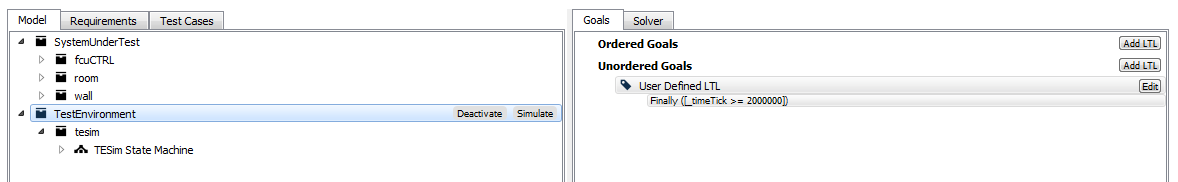
\includegraphics[width=1.0\textwidth]{roomwall/mbtconf}
    \caption{Test Goal Configuration of FCU}
    \label{fig:fcu_mbtconf}
\end{figure}

Our test results show all these implicitly covered test cases are with \T{PASS} or \T{INCONCLUSIVE} verdicts. A comparison of test results for three test configurations with the same test input sequence is displayed in Figure~\ref{fig:fcu_co-sim-result}.
\begin{figure}[htb!]
    \centering
	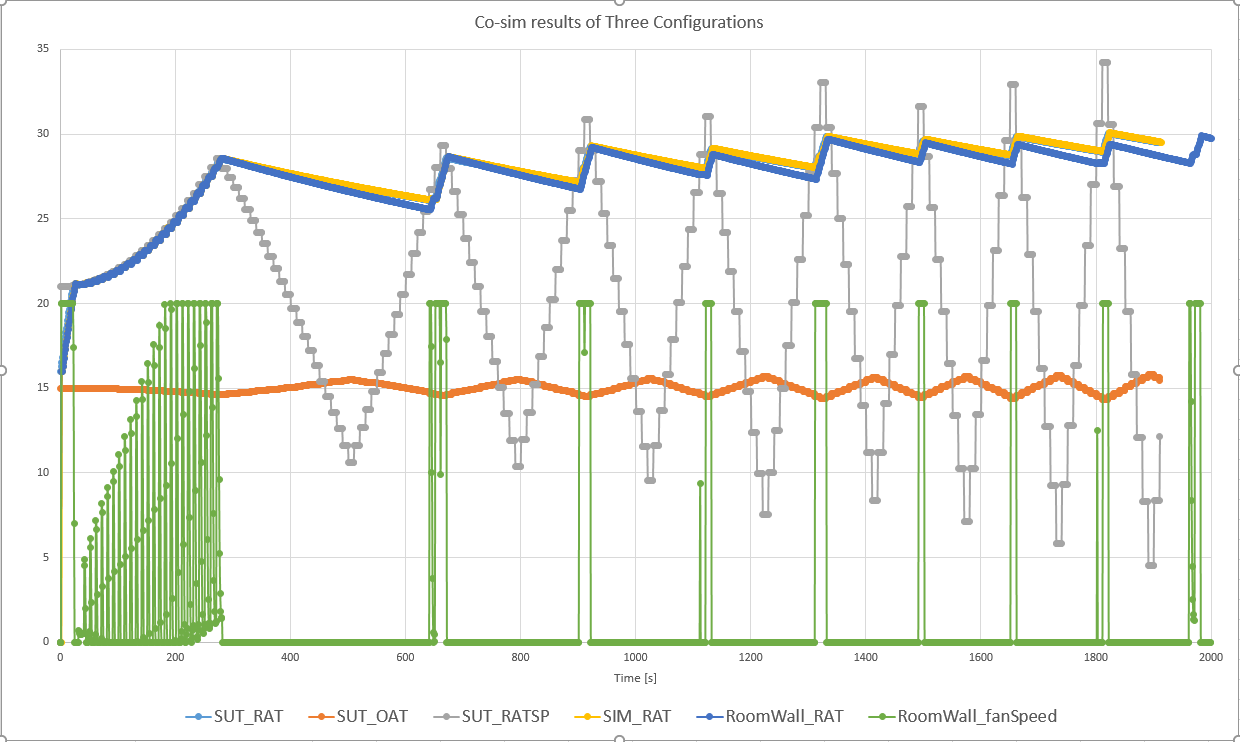
\includegraphics[width=1.0\textwidth]{test_results-20170621/fcu_co-sim-result}
    \caption{Test Results of Three Configurations}
    \label{fig:fcu_co-sim-result}
\end{figure}

From the diagram, we can see that
\begin{itemize}
    \item the change of set points will be reflected in the output $RAT$ though there are delays for the output to follow,
    \item the time to decrease temperature is longer than that to increase temperature,
    \item the fan speed is occasionally high, and most of time, the fan is inactive,
    \item the output $RAT$ from \T{SUT} almost overlaps with that of \T{SIM} (because both of them uses the Euler method for the \emph{Room} and \emph{Wall}), 
    \item the output $RAT$ from \T{SUT\_RoomWall} is slightly different from those of \T{SIM} and \T{SUT} (because the \T{RoomHeating} 20-Sim model uses the Runge Kutta 4 method).
        \begin{itemize}
            \item For \T{SUT\_RoomWall}, the room air temperature is changed faster than other two configurations.
        \end{itemize}
\end{itemize}


\subsubsection{Code Generation}

The VDM-RT model, \textbf{FCUController} can be exported from Overture as a C code FMU, in addition to the tool wrapper FMU as used above. The \emph{FCUController-SourceCode.FMU} included in this pilot is obtained directly from Overture using the ``Export Source Code FMU'' option. However, this FMU does not contain binaries for co-simulation and so one may use the \emph{FMU Builder} included in the INTO-CPS Application to compile FMUs for Windows, Mac and Linux. 

This process has been performed and the resultant FMU is included in the pilot in the FMUs folder; \emph{FCUController-Standalone.FMU}. One example experiment available is to switch this FMU for the tool wrapper version -- \emph{FCUController.FMU} -- and compare results. 
